\documentclass[a4paper,14pt]{extarticle}
\usepackage[utf8]{inputenc}
\usepackage[russian]{babel}
\usepackage{graphicx}
\usepackage[top=0.8in, bottom=0.8in, left=0.8in, right=0.8in]
{geometry}
\usepackage{pgfplots}
\usepackage{amsmath}
\usepackage{setspace}
\usepackage{titlesec}
\usepackage{float}
\usepackage{chngcntr}
\usepackage{pgfplots}
\usepackage{amsfonts}
\usepackage{pgfplotstable}
\usepackage{multirow}
\usepackage{karnaugh-map}
\usepackage{tikz,xcolor}
\usepackage{indentfirst} % Красная строка
\usepackage{listings}
\usepackage{amssymb}
\usepackage{xcolor}
\usepackage{hyperref}

\definecolor{linkcolor}{HTML}{0000FF} % цвет ссылок
\definecolor{urlcolor}{HTML}{FF00FF} % цвет гиперссылок

\hypersetup{pdfstartview=FitH, linkcolor=linkcolor,urlcolor=urlcolor, colorlinks=true}


\titleformat{\section}[hang]
  {\bfseries}
  {}
  {0em}
  {\hspace{-0.4pt}\large \thesection\hspace{0.6em}}
  
  
\titleformat{\subsection}[hang]
  {\bfseries}
  {}
  {0em}
  {\hspace{-0.4pt}\large \thesubsection\hspace{0.6em}}

%\linespread{1.3} % полуторный интервал
%\renewcommand{\rmdefault}{ftm} % Times New Roman

\newcommand{\nx}{\overline{x}}
\newcommand{\p}{0.31}
\newcommand{\scale}{1.4}

\counterwithin{figure}{section}
\counterwithin{equation}{section}
\counterwithin{table}{section}

\begin{document}
\begin{titlepage}
\centering
Санкт-Петербургский политехнический университет Петра Великого \\
\vspace{0.15cm}
Кафедра компьютерных систем и программных технологий \\
\vspace{6.5cm}

{\centering \textbf{Отчёт по лабораторной работе} \\ 
\vspace{0.15cm}
\textbf{Дисциплина}: Телекоммуникационные технологии \\
\vspace{0.15cm}
\textbf{Тема}: Сигналы телекоммуникационных
систем.\\ Преобразование
Фурье. Корреляция} \\


\vspace{6.5cm}

\begin{table}[H]
\begin{tabular}{p{\textwidth}@{}r}
{Выполнил студент гр. 33501/4} \hfill {Мальцев  М.С.} \\
{Преподаватель} \hfill {Богач Н.В.} \\
\end{tabular}
\end{table}
\vfill

{\centering Санкт-Петербург \\ 
\vspace{0.15cm}
\today}
\end{titlepage}

\tableofcontents
\newpage

\section{Цель работы}

Познакомиться со средствами генерации и визуализации простых 
сигналов. Получить представление о спектрах телекоммуникационных
сигналов.

\section{Постановка задачи}

\begin{itemize}
\item[-]
В командном окне MATLAB и в среде Simulink промоделировать 
синусоидальный и прямоугольный сигналы с различными параметрами. 
Получить их спектры. Вывести на график.

\item[-]
Выполнить расчет преобразования Фурье. Перечислить свойства
преобразования Фурье.

\item[-]
С помощью функции корреляции найти позицию синхропосылки [101] в 
сигнале [0001010111000010]. Получить пакет
данных, если известно, что его длина составляет 8 бит без
учета синхропосылки. Вычислить корреляцию прямым методом, 
используя алгоритмом быстрой корреляции, сравнить время работы 
обоих алгоритмов.

\item[-]
Быстрая корреляция
\end{itemize}

\section{Теоретический раздел}

\subsection{Сигналы}

\textbf{Сигнал} -- это физический процесс, который несёт 
некоторую информацию.\\

\textbf{Классификация сигналов:}
\begin{enumerate}
\item По физической природе носителя информации:
	\begin{itemize}
	\item электрические
	\item электромагнитные
	\item оптические
	\item акустические
	\item и другие
	\end{itemize}
\item По способу задания сигнала:
	\begin{itemize}
	\item детерминированные (описываемые аналитической функцией)
	\item случайные (для их описания используется аппарат теории 
	вероятностей)
	\end{itemize}
\item непрерывные и дискретные 
\item периодические и непериодические
\item бесконечные и конечные
\end{enumerate}

\subsection{Преобразования Фурье}

Преобразования Фурье осуществляется с помощью ряда Фурье и с 
помощью интеграла Фурье, причём первый применяется когда функция 
периодическая, а второй когда она апериодична.\\

Ряд Фурье -- представление функции f с периодом $\tau$ в виде 
ряда:
\begin{equation}
f(x) = {a_0\over 2} + \sum_{k=1}^{+\infty}A_k cos(k{2\pi\over 
\tau}x + \theta_k)
\end{equation}

Интегралы Фурье имеют вид:
\begin{equation}
F(j\omega) = \int_{-\infty}^{\infty} f(t) e^{-it\omega} dt
\end{equation}

\begin{equation}
f(t) = {{1}\over{2\pi}} \int_{-\infty}^{\infty} f(j\omega) e^{-it
\omega} d\omega
\end{equation}

Этот метод может применяться только для абсолютно интегрируемых 
функций времени, удовлетворяющих неравенству:

\begin{equation}
\int_{-\infty}^{\infty} {f(t)}^2  dt < \infty
\end{equation}

\subsection{Корреляция сигналов}

Корреляция является методом анализа сигналов. В качестве примера использования метода можно привести следующее, допустим, что имеется сигнал s(t), в котором может быть (а может и не быть) некоторая последовательность x(t) конечной длины Т, временное положение которой нас интересует. Для поиска этой последовательности в скользящем по сигналу s(t) временном окне длиной Т вычисляются скалярные произведения сигналов s(t) и x(t). Тем самым мы "прикладываем" искомый сигнал x(t) к сигналу s(t), скользя по его аргументу, и по величине скалярного произведения оцениваем степень сходства сигналов в точках сравнения. Для сигналов $s(t)$ и $x(t)$ кросс-корреляция будет вычисляться по формуле \ref{cross-corr}.

\begin{equation}
\omega(t) = s(t)\otimes x(t) \triangleq \int^{\infty}_{-\infty} s^*(\tau)\ x(\tau+t)\ d\tau
\label{cross-corr}
\end{equation}


Корреляционный анализ дает возможность установить в сигналах (или в рядах цифровых данных сигналов) наличие определенной связи изменения значений сигналов по независимой переменной, то есть, когда большие значения одного сигнала (относительно средних значений сигнала) связаны с большими значениями другого сигнала (положительная корреляция), или, наоборот, малые значения одного сигнала связаны с большими значениями другого (отрицательная корреляция), или данные двух сигналов никак не связаны (нулевая корреляция).

В варианте автокорреляции (autocorrelation) по аналогичной методике производится определение скалярного произведения сигнала s(t) с собственной копией, скользящей по аргументу. Автокорреляция позволяет оценить среднестатистическую зависимость текущих отсчетов сигнала от своих предыдущих и последующих значений (так называемый радиус корреляции значений сигнала), а также выявить в сигнале наличие периодически повторяющихся элементов.

Особое значение методы корреляции имеют при анализе случайных процессов для выявления неслучайных составляющих и оценки неслучайных параметров этих процессов.

Автокорреляционная функция (АКФ) сигнала s(t), конечного по энергии, является количественной интегральной характеристикой формы сигнала, выявления в сигнале характера и параметров взаимной временной связи отсчетов, что всегда имеет место для периодических сигналов, а также интервала и степени зависимости значений отсчетов в текущие моменты времени от предыстории текущего момента. АКФ определяется интегралом от произведения двух копий сигнала s(t), сдвинутых относительно друг друга на время $\tau$:

\begin{equation}
\omega(t) \triangleq \int^{\infty}_{-\infty} s^*(\tau)\ s(\tau+t)\ d\tau = ||s(\tau)|| \ ||s(\tau+t)|| \ cos \varphi(\tau)
\end{equation}

\section{Ход работы}

\subsection{Моделирование синусоидального сигнала}

\subsubsection{Получение непрерывного сигнала}

При открытие Simulink был выбран шаблон Simple Simulation.

\begin{figure}[H]
\center{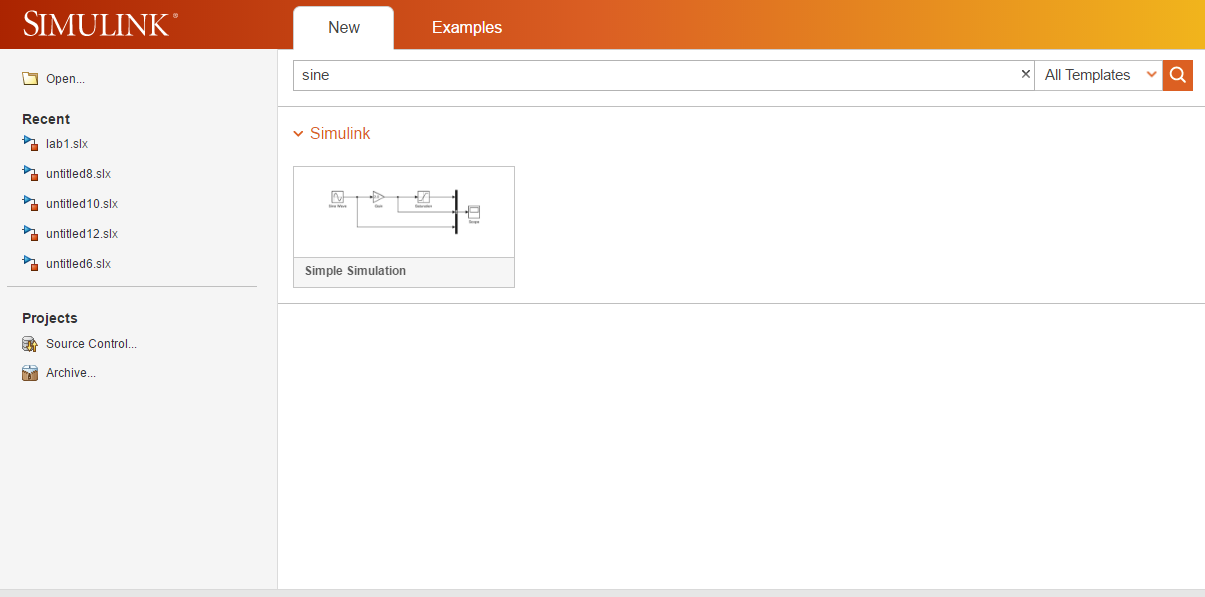
\includegraphics[width=0.82\linewidth]{img/000.png}}
\caption{Выбор шаблона в начальном окне Simulink.}
\end{figure}

Была сгенерирована схема представленная на рисунке \ref{001}.

\begin{figure}[H]
\center{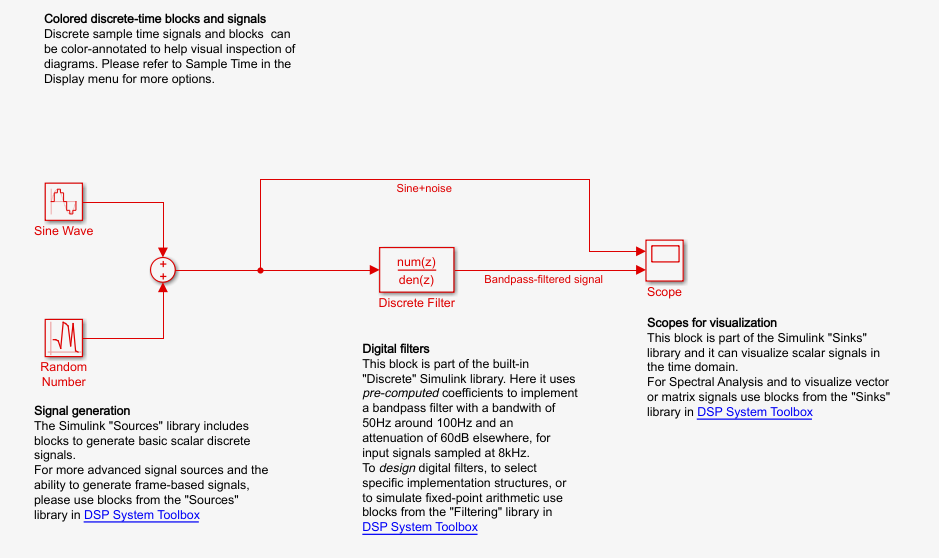
\includegraphics[width=1\linewidth]{img/001.png}}
\caption{Схема автоматически сгенерированная Simulink.}
\label{001}
\end{figure}

Краткое описание назначения элементов:
\begin{itemize}
\item \textbf{Sine Wave} задаёт синусоидальный сигнал с 
амплитудой 1 и частотой 1 rad/sec
\item \textbf{Gain} усиливает входной сигнал в 2 раза
\item \textbf{Saturation} устанавливает ограничивающие пределы 
верхний на 0.5 и нижний на -0.5\\
\end{itemize}

Таким образом, при симуляции мы должны увидеть на графике 3 
сигнала:
\begin{enumerate}
\item синусоидальный сигнал с амплитудой 1
\item синусоидальный сигнал с амплитудой 2
\item сигнал трапециевидной формы с амплитудой 0.5
\end{enumerate}

Причём, для всех сигналов должен быть одинаковый период,\\ равный 
$\sim$ 6.28 секунды.\\

При запуске симуляции получили результаты продемонстрированные на 
рисунке \ref{002}.

\begin{figure}[H]
\center{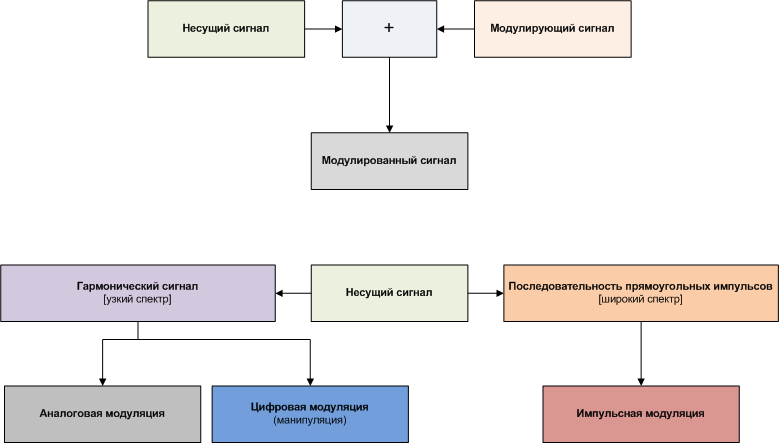
\includegraphics[width=1\linewidth]{img/002.png}}
\caption{Результат симуляция непрерывного сигнала. Окно Scope.}
\label{002}
\end{figure}

Проанализировав результаты симуляции, на соответствие ожиданиям, 
можно сделать вывод, что она выполнена правильно.

\subsubsection{Получение дискретного сигнала}

Не изменяя общую структуру, представленную на рисунке \ref{001}, 
изменим для элемента \textbf{Sine Wave} параметр $Sine \ type$ с 
$Time \ based$ на $Sample \ based$, таким образом мы сделаем 
сигнал дискретным. Установим $Samples \ per \ period$ на $20\pi$, 
$\ Sample \ time$ на $0.1$.

\begin{figure}[H]
\center{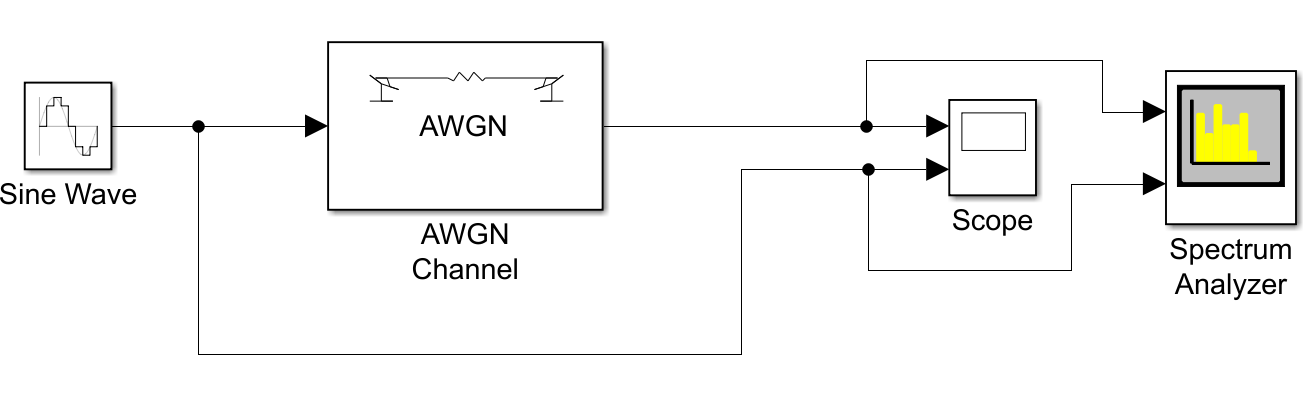
\includegraphics[width=1\linewidth]{img/003.png}}
\caption{Результат симуляция дискретного сигнала. Окно Scope.}
\label{003}
\end{figure}

На рисунке \ref{003} видно, что непрерывный сигнал стал 
дискретным, что соответствует нашим ожиданиям.

\subsubsection{Получение спектра дискретного сигнала}

Для дискретного сигнала получим его спектр. Для этого установим 
$Sample \ time$ на 0.01 и $Simulation \ stop \ time$ на 20.

\begin{figure}[H]
\center{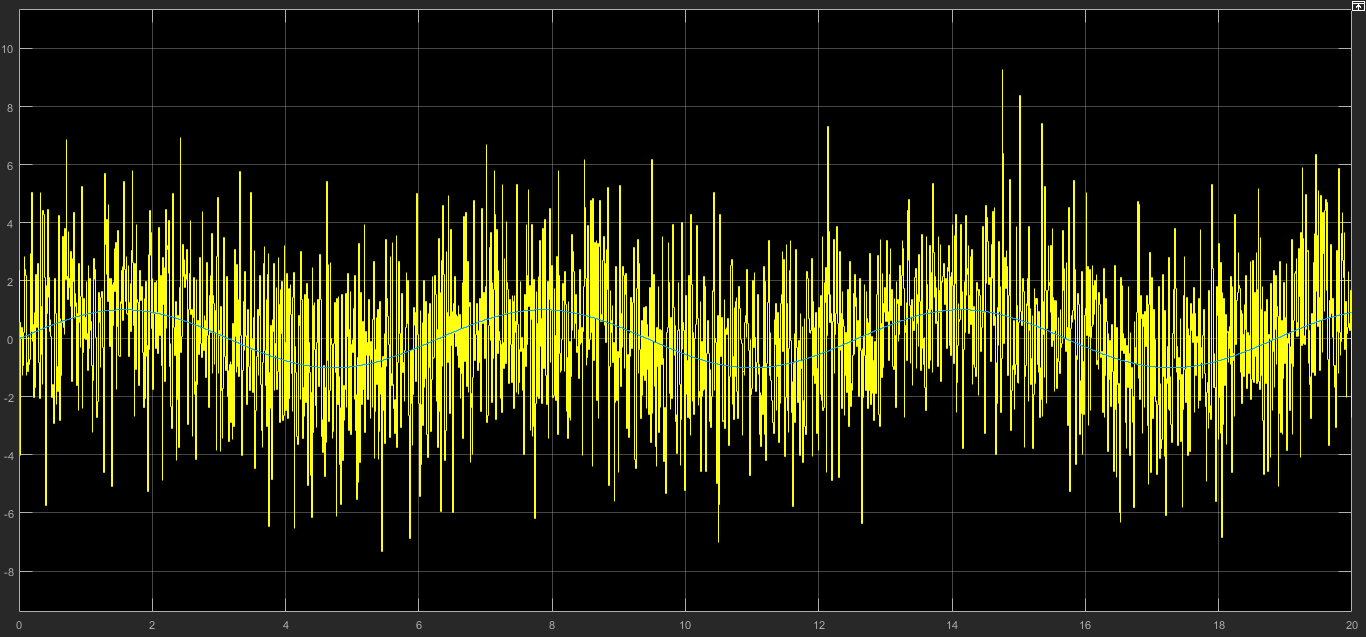
\includegraphics[width=0.65\linewidth]{img/004.png}}
\caption{Схема для исследования спектра дискретного 
синусоидального сигнала.}
\label{004}
\end{figure}

При запуске симуляции был получен результат, продемонстрированный 
на рисунке \ref{005}.

\begin{figure}[H]
\center{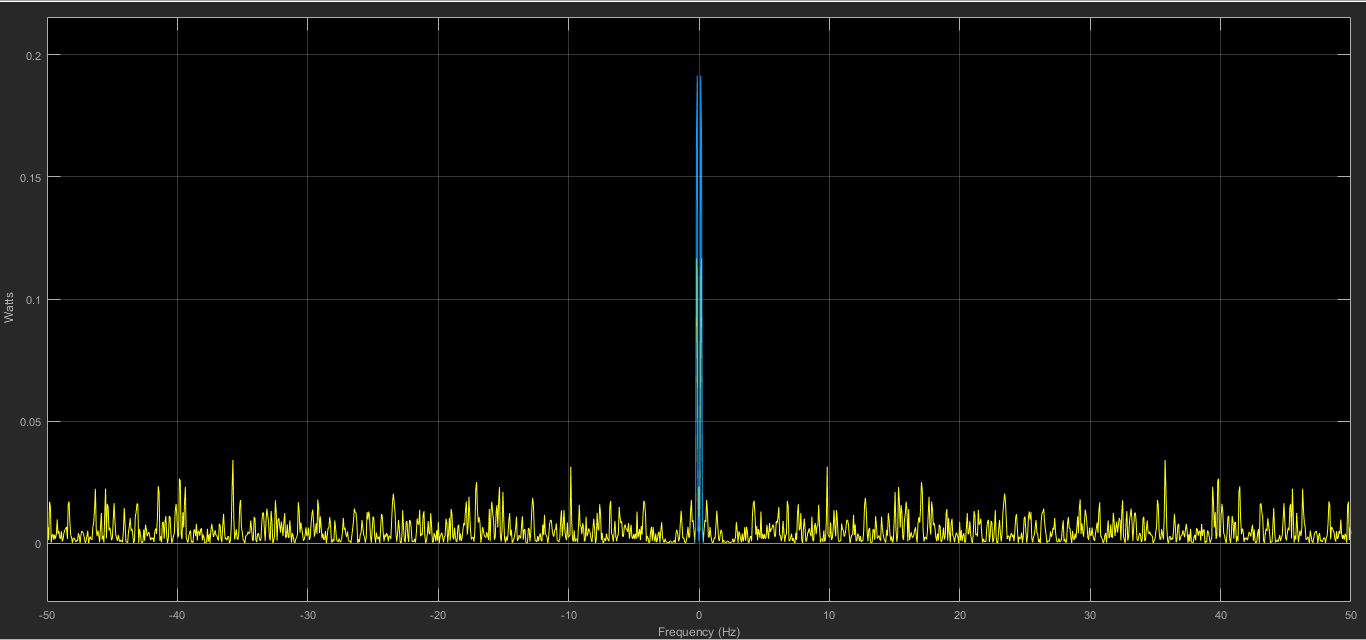
\includegraphics[width=1\linewidth]{img/005.png}}
\caption{Спектр синусоидального дискретного сигнала. Окно 
Spectrum Analyzer.}
\label{005}
\end{figure}

Изменим амплитуду входного сигнала с 1 до 5 и промодулируем 
снова.

\begin{figure}[H]
\center{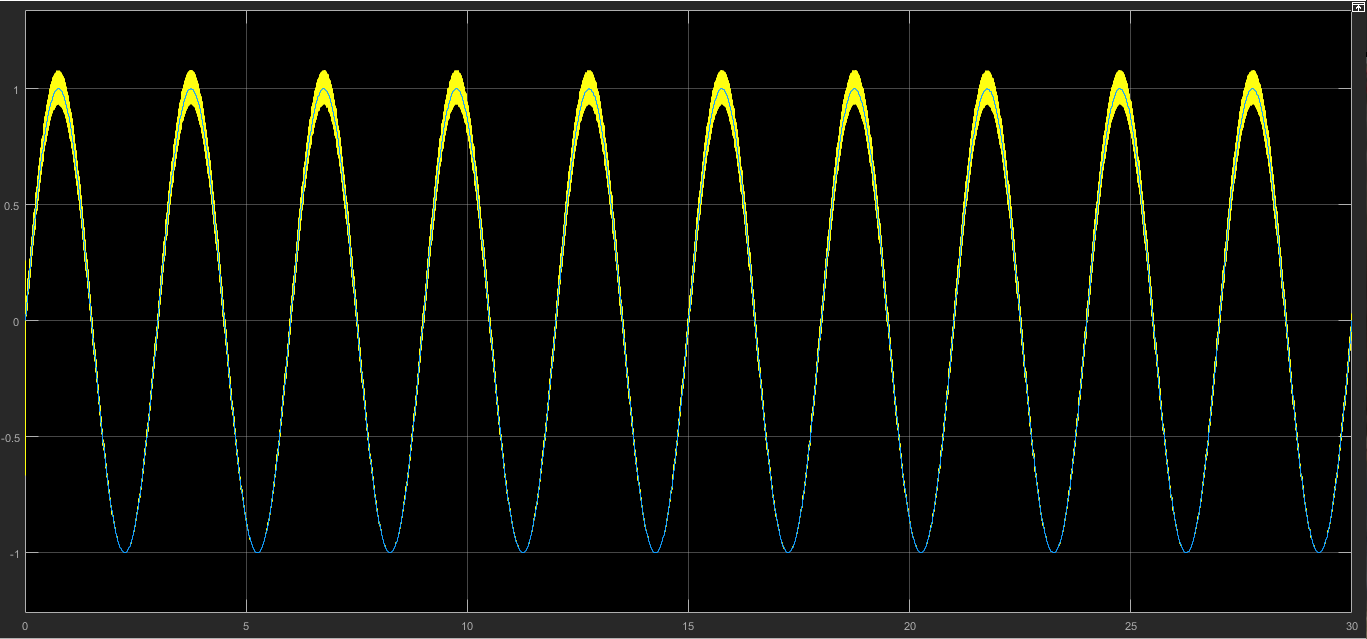
\includegraphics[width=1\linewidth]{img/006.png}}
\caption{Спектр синусоидального дискретного сигнала. Окно 
Spectrum Analyzer.}
\label{006}
\end{figure}

Изменим $Samples \ per \ period$ c $20\pi$ до $40\pi$

\begin{figure}[H]
\center{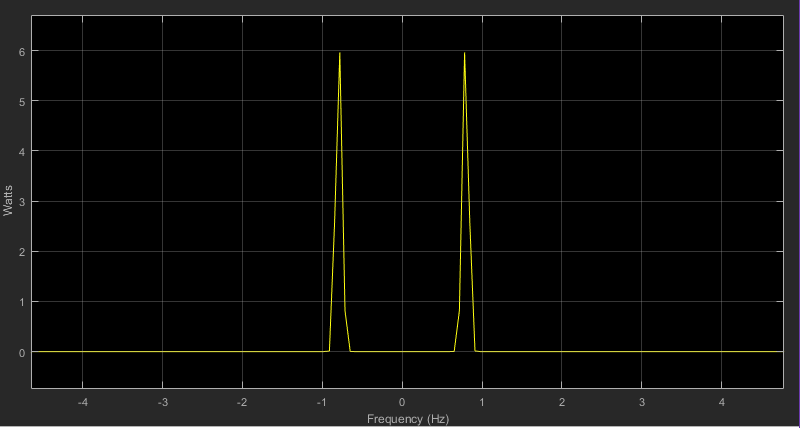
\includegraphics[width=1\linewidth]{img/007.png}}
\caption{Спектр синусоидального дискретного сигнала. Окно 
Spectrum Analyzer.}
\label{007}
\end{figure}

По полученным результатам варьирования параметров задания сигнала 
можно сделать вывод о том, что моделирование было проведено 
верно. На рисунках \ref{005}, \ref{006}, \ref{007} 
продемонстрировано, что при изменение амплитуды сигнала 
изменяется амплитуда спектра, причём нелинейно, а при изменение 
периода обратно пропорционально изменяется частота спектра.

\subsection{Моделирование прямоугольного сигнала}

\subsubsection{Получение дискретного сигнала}

Для исследования прямоугольного дискретного сигнала была введена 
схема представленная на рисунке \ref{008}. $Simulation \ stop \ 
time$ установлен на 20.

\begin{figure}[H]
\center{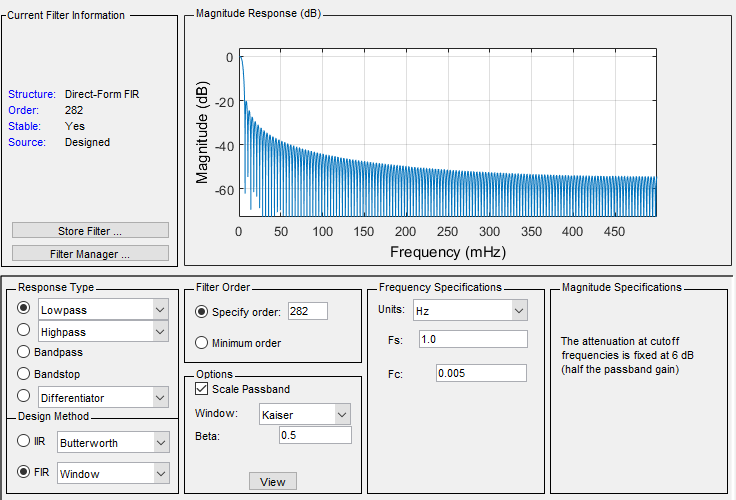
\includegraphics[width=0.6\linewidth]{img/008.png}}
\caption{Схема для исследования прямоугольного дискретного 
сигнала}
\label{008}
\end{figure}

Для \textbf{Pulse Generator} были заданы параметры представленные 
на рисунке \ref{009}

\begin{figure}[H]
\center{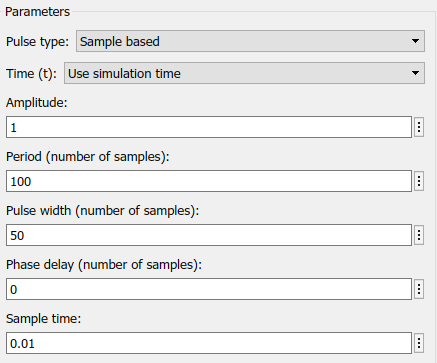
\includegraphics[width=0.6\linewidth]{img/009.png}}
\caption{Окно Block Parameters: Pulse Generator. Раздел 
Parameters.}
\label{009}
\end{figure}

После моделирования в окне Scope были получены результаты, 
продемонстрированные на рисунке \ref{010}.

\begin{figure}[H]
\center{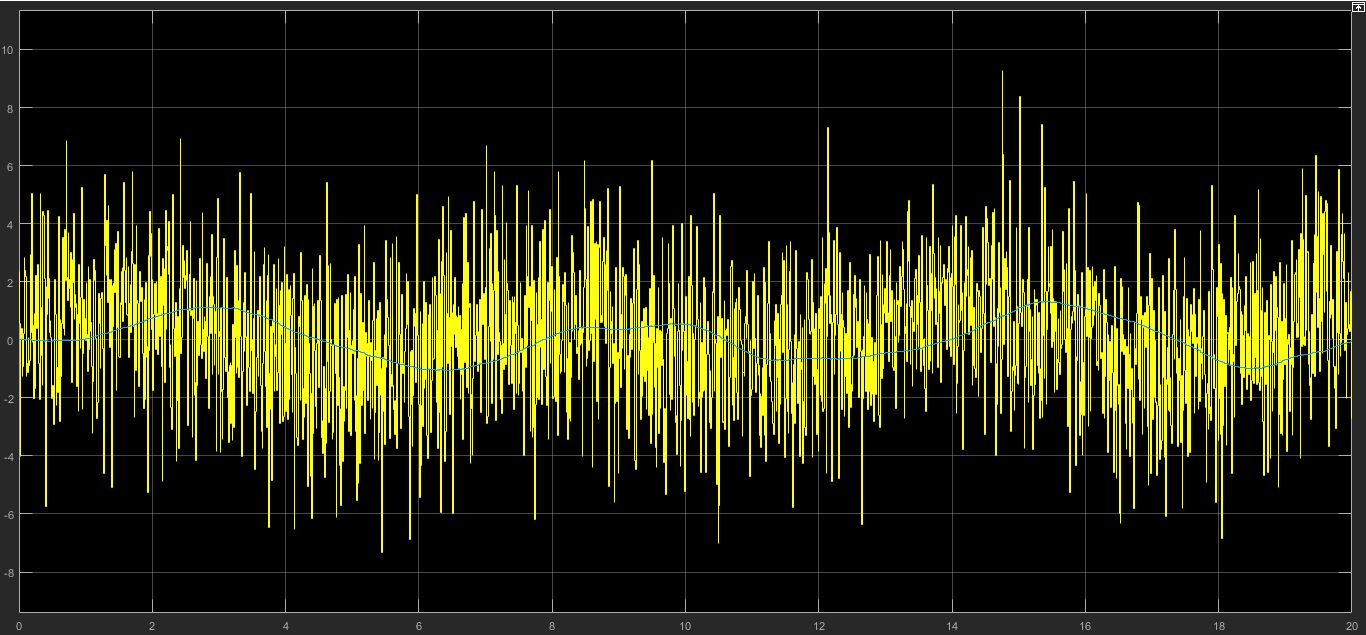
\includegraphics[width=1\linewidth]{img/010.png}}
\caption{Результаты симуляции дискретного прямоугольного сигнала. 
Окно Scope.}
\label{010}
\end{figure}

По результатам симуляции, визуально можно определить, что 
поставленная задача, смоделировать прямоугольный сигнал, 
выполнена.

\subsubsection{Получение спектра дискретного сигнала}

Для получения спектра дискретного сигнала воспользуемся схемой 
приведённой на рисунке \ref{008}.

Результаты проведённой симуляции приведены на рисунке \ref{011}.

\begin{figure}[H]
\center{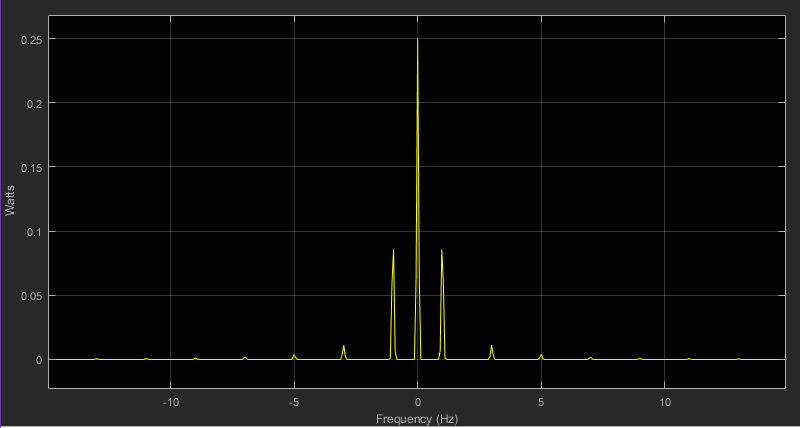
\includegraphics[width=1\linewidth]{img/011.png}}
\caption{Полученный спектр для дискретного прямоугольного 
сигнала. Окно Spectrum Analyzer.}
\label{011}
\end{figure}

Будем изменять параметры сигнала и следить за изменением спектра.

Изменим период сигнала со 100 до 75.

\begin{figure}[H]
\center{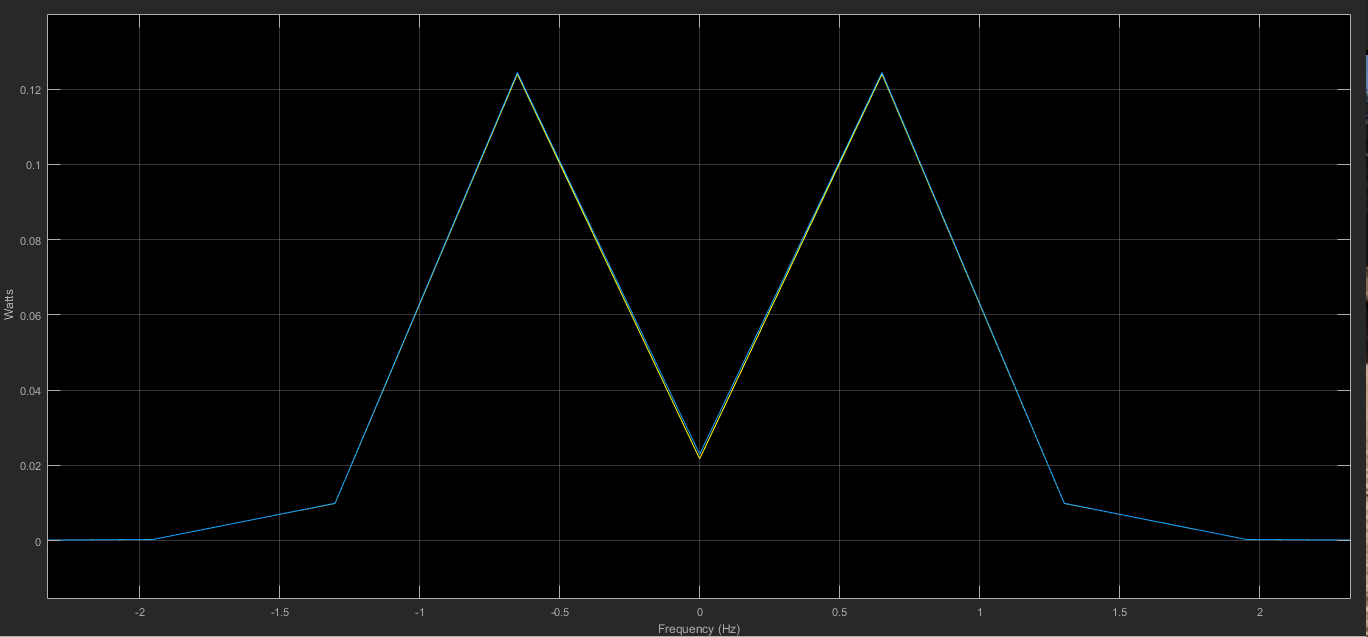
\includegraphics[width=1\linewidth]{img/012.png}}
\caption{Полученный спектр для дискретного прямоугольного 
сигнала. Окно Spectrum Analyzer.}
\label{012}
\end{figure}

Изменим длину импульса с 50 до 25.

\begin{figure}[H]
\center{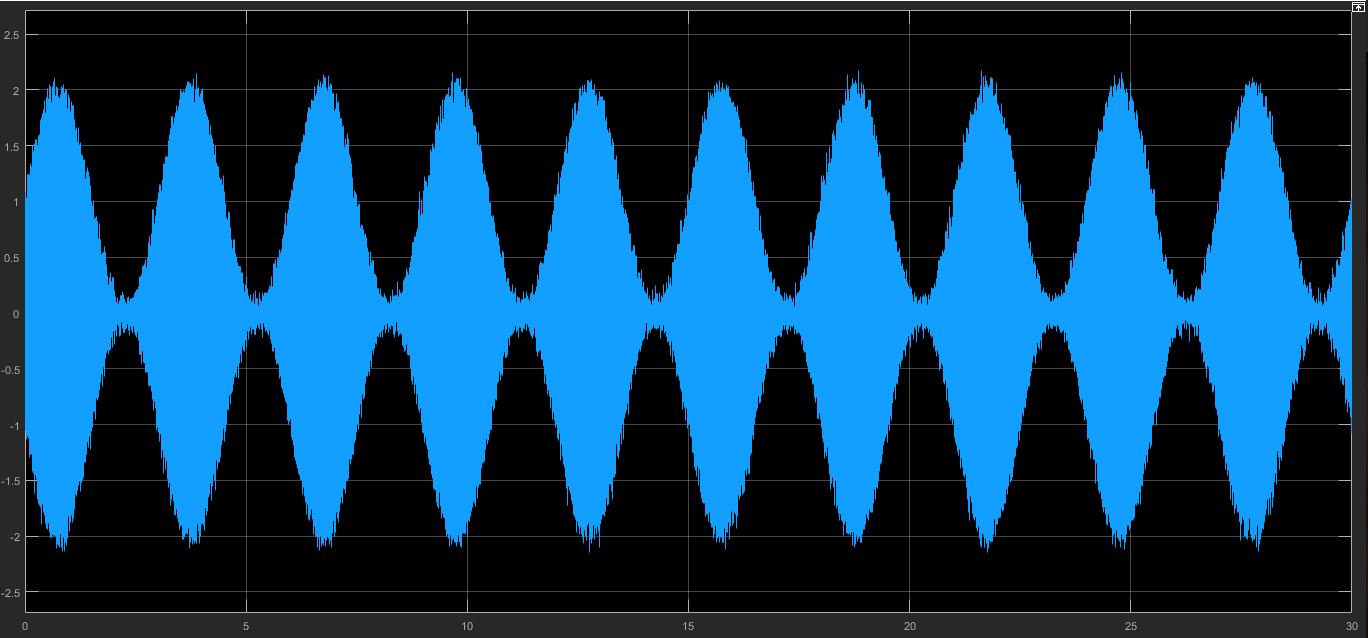
\includegraphics[width=1\linewidth]{img/013.png}}
\caption{Полученный спектр для дискретного прямоугольного 
сигнала. Окно Spectrum Analyzer.}
\label{013}
\end{figure}

Таким образом, были получены спектры различных дискретных 
прямоугольных сигналов.

\section{Корреляция сигналов}

В среде Matlab была разработана программа моделирующая передачу 2 байтового сообщения, в котором заключена 1 байтовая посылка.

Для выявления посылки было применено два метода: \textbf{ifft} и \textbf{xcorr}. Полученные результаты продемонстрированы на рисунке \ref{014}.


\begin{figure}[h]
\begin{minipage}[h]{0.49\linewidth}
\center{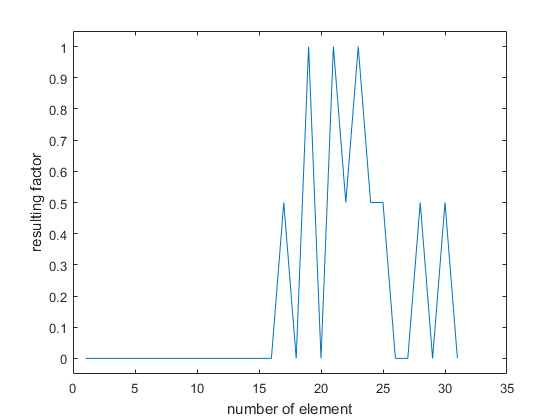
\includegraphics[width=1\linewidth]{img/014_1.png} \\ ifft}
\end{minipage}
\hfill
\begin{minipage}[h]{0.49\linewidth}
\center{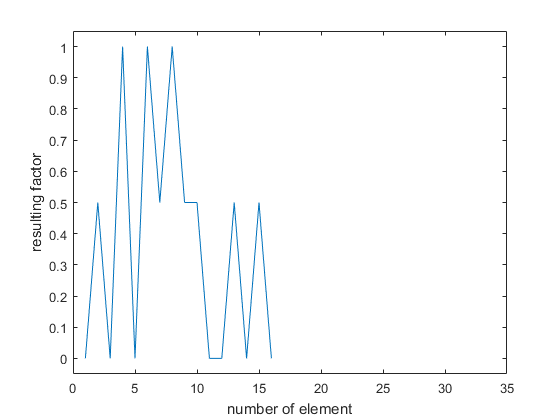
\includegraphics[width=1\linewidth]{img/014_2.png} \\ xcorr}
\end{minipage}
\caption{Результаты вычисления кросс-корреляции}
\label{014}
\end{figure}

Была разработана собственная функция \textbf{corr}, предназначенная для выявления основной части сообщения. Функция продемонстрированная на листинге \ref{corr}, была протестирована на различных входных данных листинг \ref{lab2_1}. Проверка прошла успешно.

Для сравнения времени работы функций \textbf{ifft} и \textbf{xcorr} использовалась программа с листинга \ref{lab2_2}. На рисунке \ref{015}  представлены два графика с различным шагом дискретизации. Красным обозначен -- \textbf{ifft}, синим -- \textbf{xcorr}.

\begin{figure}[H]
\begin{minipage}[h]{0.49\linewidth}
\center{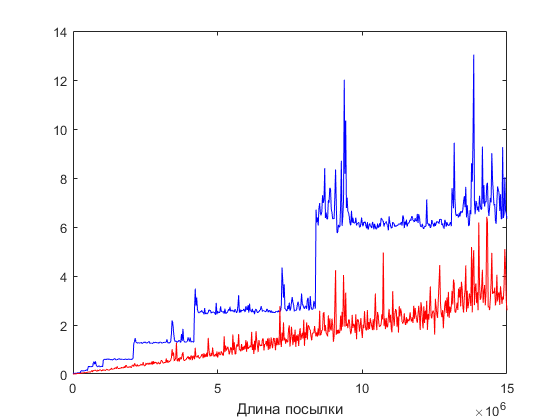
\includegraphics[width=1\linewidth]{img/015_1.png} \\ с шагом 25 000}
\end{minipage}
\hfill
\begin{minipage}[h]{0.49\linewidth}
\center{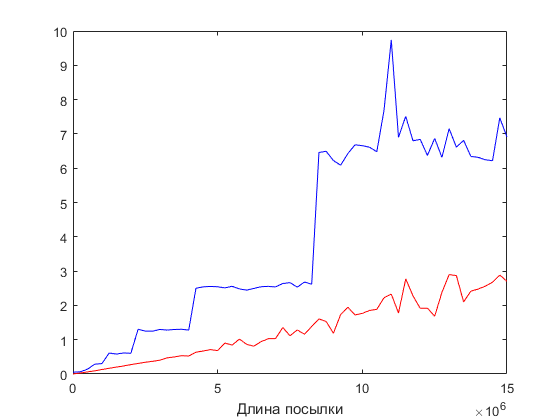
\includegraphics[width=1\linewidth]{img/015_2.png} \\ с шагом 500 000}
\end{minipage}
\caption{Время затрачиваемое на кросс-корреляцию в зависимости от длины посылки}
\label{015}
\end{figure}

На рисунке \ref{015}  продемонстрировано преимущество использования \textbf{ifft} над \textbf{xcorr}.



\section{Выводы}

Сигналы используются для передачи информации. Сигналы 
различаются по природе носителя информации, по способу 
задания сигнала, по непрерывности, по периодичности и по 
конечности.

Они могут быть представлены как во временной, так и в 
частотной области. Переход от одного представления к другому 
можно осуществить с помощью преобразований Фурье. Преобразование применяют потому что при анализе сигналов для одних удобнее временное отображение, а для других частотное.

Корреляционный анализ дает возможность установить в сигналах наличие связи. Методы корреляции активно применяются при анализе случайных процессов для выявления неслучайных составляющих и оценки неслучайных параметров этих процессов.


\section{Используемые материалы}

\begin{enumerate}
\item \href{http://www.ee.ic.ac.uk/hp/staff/dmb/courses/E1Fourier/00800_Correlation.pdf}{Correlation (E1.10 Fourier Series and Transforms)}

\item \href{https://en.wikipedia.org/wiki/Fourier_transform}{Fourier transform (Wikipedia)}

\item \href{https://en.wikipedia.org/wiki/Signal}{Signal (Wikipedia)}

\item \href{http://bourabai.kz/signals/ts08.htm}{Корреляция сигналов (Давыдов А.В. Теория сигналов и линейных систем)}
\end{enumerate}

\newpage

\section{Приложение}

\lstinputlisting[language=matlab, frame=single, caption=Программа сравнения скорости работы функций, label=lab2_2]{../lab2_2.m}

\newpage

\lstinputlisting[language=Matlab, frame=single, caption=Программа тестирования функции corr, label=lab2_1]{../lab2_1.m}

\newpage

\lstinputlisting[language=Matlab, frame=single, caption=Функция для выявления основной части сообщения, label=corr]{../corr.m}

\end{document}
